%Dokumenteinstellungen und Anpassungen
%Dokumentenklasse "scrbook" - Erweitert um den Verweis auf die Verzeichnisse und Texteigenschaften
\documentclass[ 12pt, a4paper, oneside, parskip=half, listof=totoc, bibliography=totoc, numbers=noendperiod,ngerman]{scrreprt}


%Anpassung der Seitenränder (Standard bottom ca. 52mm anbzüglich von ca. 4mm für die nach oben rechts gewanderte Seitenzahl)
\usepackage[bottom=48mm,left=25mm,right=25mm]{geometry}

%Tweaks für scrbook
\usepackage{scrhack}

%Blindtext
%\usepackage{blindtext}

%Erlaubt unteranderem Umbrücke captions
\usepackage{caption}
\usepackage{derivative}
%Stichwortverzeichnis
\usepackage{imakeidx}
\usepackage{amsmath}
%Kompakte Listen
\usepackage{paralist}
% Multiline comments
\usepackage{comment}
%Zitate besser formatieren und darstellen
\usepackage{epigraph}

%Glossar, Stichworverzeichnis (Akronyme werden als eigene Liste aufgeführt)
\usepackage[toc, acronym]{glossaries} 

%Anpassung von Kopf- und Fußzeile
%beinflusst die erste Seite des Kapitels
\usepackage[automark,headsepline]{scrlayer-scrpage}
\automark{chapter}
\ihead{\leftmark}
\chead{}
\ohead{\thepage}
\ifoot*{}
\cfoot[\thepage]{}
\cfoot*{}
\ofoot*{\thepage}
\ofoot{}
\pagestyle{scrheadings}


%Auskommentieren für die Verkleinerung des vertikalen Abstandes eines neuen Kapitels
%\renewcommand*{\chapterheadstartvskip}{\vspace*{.25\baselineskip}}

%Zeilenabstand 1,5
\usepackage[onehalfspacing]{setspace}

%Verbesserte Darstellung der Buchstaben zueinander
\usepackage[stretch=10]{microtype}

%Deutsche Bezeichnungen für angezeigte Namen (z.B. Innhaltsverzeichnis etc.)
\usepackage[ngerman]{babel}

%Unterstützung von Umlauten und anderen Sonderzeichen (UTF-8)
\usepackage{lmodern}
\usepackage[utf8]{luainputenc}
\usepackage[T1]{fontenc}

%Einfachere Zitate
\usepackage{epigraph}

%Unterstützung der H positionierung (keine automatische Verschiebung eingefügter Elemente)
\usepackage{float} 

%Erlaubt Umbrüche innerhalb von Tabellen
\usepackage{tabularx}

%Erlaubt Seitenumbrüche innerhalb von Tabellen
\usepackage{longtable}

%Erlaubt die Darstellung von Sourcecode mit Highlighting
\usepackage{listings}

%Definierung eigener Farben bei nutzung eines selbst vergebene Namens
\usepackage[table,xcdraw]{xcolor}

%Vektorgrafiken
\usepackage{tikz}

%Grafiken (wie jpg, png, etc.)
\usepackage{graphicx}

%Grafiken von Text umlaufen lassen
\usepackage{wrapfig}

%Ermöglicht Verknüpfungen innerhalb des Dokumentes (e.g. for PDF), Links werden durch "hidelink" nicht explizit hervorgehoben
\usepackage[hidelinks,german]{hyperref}
\usepackage{cleveref}
\usepackage{siunitx}
%Einbindung und Verwaltung von Literaturverzeichnissen
\usepackage{csquotes} %wird von biber benötigt
\usepackage[style=ieee, backend=biber, bibencoding=ascii]{biblatex}
\addbibresource{references/references.bib}

%Anpassung der Überschriften
\addtokomafont{disposition}{\rmfamily}

%Zusätzliche Farben
\definecolor{darkgreen}{RGB}{0,100,0}

%Umbenennungen
\renewcommand{\lstlistlistingname}{Quelltextverzeichnis}

%Pluszeichen in der Referenc beim zitieren ausblenden
\renewcommand*{\labelalphaothers}{}

%Anpassugen zur Quelltextdarstellung, kann bei Bedarf überschrieben werden (z.B. wenn unterschiedliche Sprachen zum Einsatz kommen)
\renewcommand{\lstlistingname}{Codeauszug}
\lstset{
	language=Java,
	numbers=left,
	columns=fullflexible,
	aboveskip=5pt,
	belowskip=10pt,
	basicstyle=\small\ttfamily,
	backgroundcolor=\color{black!5},
	commentstyle=\color{darkgreen},
	keywordstyle=\color{blue},
	stringstyle=\color{gray},
	showspaces=false,
	showstringspaces=false,
	showtabs=false,
	xleftmargin=16pt,
	xrightmargin=0pt,
	framesep=5pt,
	framerule=3pt,
	frame=leftline,
	rulecolor=\color{green},
	tabsize=2,
	breaklines=true,
	breakatwhitespace=true,
	prebreak={\mbox{$\hookleftarrow$}}
}

%Anpassungen für das Abkürzungsverzeichnis
\newglossarystyle{dottedlocations}{%
	\renewcommand*{\glossaryentryfield}[5]{%
		\item[\glsentryitem{##1}\glstarget{##1}{##2}] \emph{##3}%
		\unskip\leaders\hbox to 2.9mm{\hss.}\hfill##5}%
	\renewcommand*{\glsgroupskip}{}%
}

%Titelformen - gewünschtes Layout einkommentieren

%%Graduation
\makeatletter

\newcommand*{\gradeType}[1]{\gdef\@gradeType{#1}}
\newcommand*{\firstExaminer}[1]{\gdef\@firstExaminer{#1}}
\newcommand*{\secondExaminer}[1]{\gdef\@secondExaminer{#1}}
\newcommand*{\matrikelnr}[1]{\gdef\@matrikelnr{#1}}
\newcommand*{\submitDate}[1]{\gdef\@submitDate{#1}}

\renewcommand*{\maketitle}{
	\begin{titlepage}
		\newgeometry{left=2.5cm,right=2.5cm,top=9.0cm,bottom=2.5cm}
		\begin{center}
			\vfill
			{\Large \@title\par}
			\vskip 0.5cm
			{\large \bfseries Abschlussarbeit\par}
			\vskip 0.5cm
			{\large zur Erlangung des akademischen Grades\\ \bfseries \@gradeType}
			\vskip 0.5cm
			{\large an der}
			\vskip 0.5cm
			{\large Hochschule für Technik und Wirtschaft Berlin\\ Fachbereich Wirtschaftswissenschaften II\\ Studiengang Angewandte Informatik}
			\vfill
			\begin{flushleft}
				\begin{tabular}[t]{rl}
					1. Prüfer: &\@firstExaminer\\
					2. Prüfer: & \@secondExaminer\\
					\\
					Eingereicht von: &\@author\\
					Matrikelnummer: & \@matrikelnr\\
					Datum der Abgabe: & \@submitDate
				\end{tabular}
			\end{flushleft}
		\end{center}
		\restoregeometry
	\end{titlepage}
}
\makeatother
\gradeType{Master of Science (M.Sc.)}
\secondExaminer{Max Mustermann}

%Research paper
%\include{titles/research_papger}
%\subTitle{Ein optionaler Untertitel der Arbeit}
%\researchPart{A}

%Angaben zur Arbeit und dem Author (von beiden Layouts genutzt)
\title{Dies ist der Titel der Abschlussarbeit der sich auch über mehrere Zeilen erstrecken kann}
\author{Max Mustermann}
\matrikelnr{s0000000}
\submitDate{25.04.2017}
\firstExaminer{Max Mustermann}

%Verzeichnisse generieren
\makeglossaries
\loadglsentries{references/glossary_acronyms.tex}
\setacronymstyle{long-short}

\makeindex[columns=2, title=Stichwortverzeichnis, options= -s resources/styles/indexstyle.ist, intoc]
\indexsetup{level=\chapter*,toclevel=chapter}

%Start des Inhalts
\begin{document}

%Notwendiger Workaround
\pagenumbering{alph}

%Deckblatt erzeugen
\maketitle

\pagenumbering{Roman}

%\chapter*{Vorwort}
\blindtext \clearpage
%\chapter*{Abstract}

\blindtext \clearpage

%Inhaltsverzeichnis
\tableofcontents \newpage

%Hauptteil
\pagenumbering{arabic}
\chapter{Einleitung}
Die allgemeine DGL ist gegeben durch:
\begin{equation}
	\frac{\partial u}{\partial t}= D\cdot\frac{\partial ^2 u }{\partial z^2}-(k1+k2\cdot N_D)\cdot u -k2u^2 +s(t,z)
\end{equation}

Zu erst wird die stationäre DGL ohne zeitliche Abhängigkeit betrachtet:

\begin{equation}
	D\cdot \frac{du}{dt} -\left( k_1 +k_2 N_D\right)\cdot u-k_2\cdot u^2=-s(z)
\end{equation}


 \clearpage
\chapter{Finite Differenzen der stationären Gleichung}
Im folgendem Kapitel soll die stationäre Verteilung der Ladungsträger bei
kontinuierlicher Bestrahlung modelliert werden.
Dadurch kann die zeitliche Abhängigkeit vernachlässige werden ($\frac{\partial
		u}{\partial t}=0$)

Die allgemeine DGL ist gegeben durch:
\begin{equation}
	\frac{\partial u}{\partial t}= D\cdot\frac{\partial ^2 u }{\partial
		z^2}-(k1+k2\cdot N_D)\cdot u -k2u^2 +s(t,z)
\end{equation}

\begin{conditions}
	s(t,z)	   &  Ladungsträgerdichte durch Bestrahlung \\
	D     &  Diffusionskonstante \\
	N_D &  Dotierungsdichte \\
	k1,k2 &  Rekombinationskonstanten \\
	\alpha & Absorptionskonstante\\
	S_L,S_R  & Rekombinationsraten an den jeweiligen Grenzschichten
\end{conditions}

Mit $\frac{\partial u}{\partial t}=0$ folgt die stationäre Gleichung:

\begin{equation}\label{eq:stationDGL}
	D\cdot \pdv[2]{u}{z} -\left( k_1 +k_2 N_D\right)\cdot u-k_2\cdot
	u^2=-s(z), \quad 0 <z<d
\end{equation}

mit den Randbedingungen:

\begin{equation}\label{eq:randbedingungen}
	D\cdot \frac{\partial u}{\partial z}(0)=S_Lu(0),\quad D\frac{\partial
		u}{\partial z}(d)=-S_Ru(d)
\end{equation}

\section{Lineare stationäre Gleichung}
Im Folgendem Kapitel soll nur der in u lineare Anteil der stationären,
zeitunabhängigen Gleichung (Eq. \ref{eq:stationDGL}) ohne den quadratischen
Term $-k_2u^2$ behandelt werden\cite{Prof.Dr.AndreasZeiser.April2021}.

\begin{mybox}
	\textbf{Aufgabe 1.} Erarbeiten Sie sich Abschnitt 8.8 aus
	\cite{Atkinson.2004} und beschreiben Sie Ihr Vorgehen für die Anwendung der
	Methode auf Gleichung.\cite{Prof.Dr.AndreasZeiser.April2021}
\end{mybox}

Mit der Methode der finiten Differenzen für
Zweipunkt-Grenzwertprobleme, beschrieben in \cite[p. 442]{Atkinson.2004},
können lineare Differenzialgleichungen zweiter Ordnung gelöst werden. Es werden
dabei die Ableitungen der Gleichung durch finite Differenzen substituiert, um
eine diskretisierte Gleichung zu erhalten.
Als Ergebnis erhält man eine Matrix, mit der sich die zeitabhängige
Stelle der Leitungsträgerdichte $u_i$ mathematisch beschreiben lassen.

Für diese Methode sind drei Schritte notwendig:
\begin{enumerate}
	\item Diskretisierung eines Bereiches ($z\in [0,d]$) der
	      Funktion in $M$ gleich große Intervalle der Länge $h=\frac{(d-0)}{N}$
	      (\cref{fig:bsp_knotenpunkte})
	\item Diskretisierung der Differenzialgleichung an den
	      Knotenpunkten mit Approximation der Ableitung
	      (\cref{eq:approx_first_order,eq:approx_second_order})
	\item Diskretisierung der Randbedingung und Aufstellung eines
	      Gleichungssystemes durch Eliminierung von $u_{-1}$ und $u_{N+1}$
\end{enumerate}

\begin{mybox}
	\textbf{Aufgabe 2.} Leiten Sie analog zu Gleichung (8.128) die
	Gleichungen für die gesuchten Werte  $u_0, u_1, \dots , u_N$ an den Punkten
	$z_0,\dots, z_N$ her. Die Gleichungen enthalten $u_1$ und $u_\mathrm{N+1}$, die
	im nächsten Schritt eliminiert werden. Verwenden Sie dabei die Abkürzung $ s_i
		= s(z_i)$.\cite{Prof.Dr.AndreasZeiser.April2021}
\end{mybox}

\begin{figure}[htb]
	\centering
	\begin{tikzpicture}
		\begin{axis}[
				axis x line = middle,
				axis y line = middle,
				xmin=-1,
				xmax=5,
				ymin=-5,
				ymax=20,
				xtick={-1,0,1,2,3,4,5},
				ytick={-5,0,5,10,15,20},
				xticklabels={$z_{-1}$,$z_0$,$z_1$,$z_2$,$z_3$,$z_N$}
			]
			\addplot[domain=-1:5]{x^2-x+10};
			\draw [dashed] (axis cs:1,1^2-1+10) -- (axis cs:1,0);
			\draw [dashed] (axis cs:2,2^2-2+10) -- (axis cs:2,0);

			\draw
			[thick,decoration={brace,mirror,raise=2pt},decorate]
			(axis cs:1,0) --
			node[below=7pt] {$h$}
			(axis cs:2,0);
		\end{axis}
	\end{tikzpicture}
	\caption{Beispieldarstellung: Knotenpunkte mit Schrittweite $h$}
	\label{fig:bsp_knotenpunkte}
\end{figure}

Stationäre Differenzialgleichung(\cref{eq:stationDGL}) ohne den quadratischen
Term $-k^2u^2$:
\begin{equation}\label{eq:linearDGL}
	D \pdv[2]{u}{z} -ku=-s(z), \quad 0 <z<d
\end{equation}
mit $k=k_1+k_2\cdot N_D$.

\begin{align*}
	k   & =k_1+k_2*N_D   \\
	s_i & = s(z_i)       \\
	u_i & \approx u(z_i)
\end{align*}
\begin{conditions}
	u_i & Approximierte Ladungsträgerdichte an den Stellen $z_i$ \\
	s_i & Ladungsträgerdichte die durch externe Bestrahlung an den Stellen
	$z_i$ erzeugt wird
\end{conditions}

Approximation der Ableitung erster Ordnung:
\begin{equation}\label{eq:approx_first_order}
	\frac{\partial u}{\partial z} = \frac{u_{i+1} - u_{i-1}}{2h}
\end{equation}
Approximation der Ableitung zweiter Ordnung:
\begin{equation}\label{eq:approx_second_order}
	\frac{\partial ^2 u }{\partial z^2} = \frac{u_{i+1} - 2\cdot u_i +
		u_{i-1}}{h^2} \quad i=1,2,\dots,N
\end{equation}

Durch Einsetzen von \cref{eq:approx_second_order} in \cref{eq:linearDGL} erhält
man:
\begin{equation}\label{eq:stationare_approx}
	D\cdot\frac{u_{i+1} - 2\cdot u_i + u_{i-1}}{h^2} -k\cdot u_i = -s_i
\end{equation}

\begin{qed}
	Nun wird nach der Variable $u_i$ sortiert und folgende Gleichung aufgestellt:
	\begin{equation}
		\frac{D}{h^2}\cdot u_{i-1} - \frac{2D+kh^2}{h^2}\cdot u_i +
		\frac{D}{h^2}\cdot u_{i+1} = -s_i
	\end{equation}
\end{qed}

\begin{mybox}
	\textbf{Aufgabe 3.}	Approximieren Sie die ersten Ableitungen an den
	Randbedingungen:

	\begin{equation}
		\tcbhighmath{	D\cdot \frac{\partial u}{\partial z}(0)=S_Lu(0),\quad
			D\frac{\partial u}{\partial z}(d)=-S_Ru(d)}
	\end{equation}
	durch:

	\begin{equation}
		\tcbhighmath{	u'(0) \approx \frac{u_1-u_{-1}}{2h}, \quad u'(d)
		\approx \frac{u_{N+1}-u_{N-1}}{2h}}
	\end{equation}

	und lösen Sie die Gleichungen nach $u_1$ bzw. $u_N+1$ auf. Setzen Sie
	diese Ausdrücke in die Gleichungen für die Knoten $z_0$ und $z_N$ der letzten
	Teilaufgabe ein.
\end{mybox}

Erste Randbedingung:

\begin{equation}
	D\cdot \frac{\partial u}{\partial z}(0)=S_Lu(0)
\end{equation}

\begin{equation}
	\frac{\partial u(0)}{\partial z}=\frac{S_Lu(0)}{D}
\end{equation}
Mit der Approximation der Ableitung erster Ordnung
(\cref{eq:approx_first_order}):
\begin{equation}
	\frac{S_Lu_0}{D} = \frac{u_1-u_{-1}}{2h}
\end{equation}

\begin{equation}
	u_0 = D\cdot \frac{u_1-u_{-1}}{2h\cdot S_\mathrm{L}}
\end{equation}

\begin{equation}
	u_0 = \frac{D}{2h\cdot S_L} \cdot u_1 - \frac{D}{2h\cdot S_L} \cdot
	u_{-1}
\end{equation}

\begin{qed}
	\textbf{Damit folgt für $u_{-1}$:}
	\begin{equation}\label{eq:rand_u-1}
		u_{\text{-}1} = u_1 - \frac{2h\cdot S_L}{D} \cdot u_0
	\end{equation}
\end{qed}

Zweite Randbedingungen:

\begin{equation}
	D\frac{\partial u}{\partial z}(d)=-S_Ru(d)
\end{equation}

\begin{equation}
	\frac{\partial u}{\partial z}(d)=-S_Ru(d)/D
\end{equation}
Durch Approximation der Randbedingung folgt:
\begin{equation}
	\frac{-S_R}{D}\cdot u_\mathrm{N} =
	\frac{u_{\mathrm{N}+1}-u_{\mathrm{N}-1}}{2h}
\end{equation}

\begin{equation}
	u_\mathrm{N} = D\cdot \frac{u_{N+1}-u_{N-1}}{-2hS_R}
\end{equation}

\begin{equation}
	u_\mathrm{N} = \frac{D}{-2hS_R} \cdot u_{N+1} - \frac{D}{-2hS_R} \cdot
	u_{\mathrm{N}-1}
\end{equation}

\begin{qed}
	\textbf{Damit folgt für $u_{\mathrm{N}+1}$}:
	\begin{equation}\label{eq:approx_RN}
		u_{N+1} =u_{\mathrm{N}-1} -\frac{2\cdot h\cdot S_R}{D} \cdot
		u_\mathrm{N}
	\end{equation}
\end{qed}

Im folgendem werden die Approximationen der Randbedingungen in die stationäre,
diskretisierte DGL (\cref{eq:stationare_approx}) eingesetzt. Dazu wird die
Diskretisierung zunächst an die Randbedingungen angepasst:
\begin{equation}
	\begin{split}
		Z_N&: \quad	D\cdot
		\frac{u_{N+1}-2u_\mathrm{N}+u_{N-1}}{h^2}-ku_N=-s_N \\
		Z_0&: \quad D\cdot \frac{u_{1}-2u_0+u_{-1}}{h^2}-ku_0=-s_0
	\end{split}
\end{equation}
mit der Approximation der Randbedingung \cref{eq:approx_RN,eq:rand_u-1} folgt:

\begin{equation}
	\begin{split}
		Z_N: \quad	D\cdot
		\frac{u_{\mathrm{N}-1}-\frac{2\cdot h\cdot S_R}{D} \cdot u_\mathrm{N}
		-2u_\mathrm{N}+u_{\mathrm{N}-1}}{h^2}-ku_N=-s_N \\
		\frac{-2hS_R-2D}{h^2}\cdot
		u_\mathrm{N}+\frac{2D}{h^2}\cdot u_{N-1}-ku_\mathrm{N}=-s_\mathrm{N}\\
		\frac{2D}{h^2}\cdot
		u_{N-1}-\frac{2hS_R+2D+kh^2}{h^2}\cdot u_\mathrm{N}=-s_\mathrm{N}
	\end{split}
\end{equation}

\begin{equation}
	\begin{split}
		Z_0: \quad	D\cdot \frac{u_1-2u_0+u_1-\frac{2\cdot h\cdot
				S_L}{D} \cdot u_0 }{h^2}-ku_0=-s_0\\
		\frac{2D}{h^2}\cdot u_1 - \frac{2D+2h\cdot
			S_\mathrm{L}+kh^2}{h^2}\cdot u_0=-S_0
	\end{split}
\end{equation}

\begin{qed}
	Es ergibt sich der Wert für $Z_0$ damit zu:
	\begin{equation}
		\tcbhighmath{Z_0: \quad \frac{2D}{h^2}\cdot u_1 -
			\frac{2D+2h\cdot S_\mathrm{L}+kh^2}{h^2}\cdot u_0=-s_0}
	\end{equation}
	Es ergibt sich der Wert für $Z_\mathrm{N}$ damit zu:
	\begin{equation}
		\tcbhighmath{Z_N: \quad \frac{2D}{h^2}\cdot
			u_{N-1}-\frac{2hS_R+2D+kh^2}{h^2}\cdot u_\mathrm{N}=-s_\mathrm{N}}
	\end{equation}

\end{qed}

\begin{mybox}
	\textbf{Aufgabe 4.} Stellen Sie das lineare Gleichungssystem für die
	Größen analog zu Gleichung (8.133) in \cite{Atkinson.2004} und folgende dar:
	\begin{equation}\label{eq:lgs}
		\mathbf{A} u = \mathbf{b},\quad \mathbf{u} = [u_i],\quad
		\mathbf{b} = [b_i]
	\end{equation}

	Ordnen Sie die Gleichungen analog zu den Knotenpunkten.
\end{mybox}

Mit Hilfe der Matrixform $\mathbf{A} u =\mathbf{ b} $ lässt sich dieses
Gleichungssystem mit Hilfe von Matlab lösen. Dazu wird die Koeffizientenmatrix

\begin{equation}
	\mathbf{A}=	\begin{bmatrix}
		-\frac{2hS_\mathrm{L}+2D+kh^2}{h^2} & \frac{2D}{h^2}        &               &               &                       &
		\\
		\frac{D}{h^2}                       & - \frac{2D+kh^2}{h^2} & \frac{D}{h^2} &               &                       &
		\\
		\ddots                              & \ddots                & \ddots        & \ddots        &                       &                            \\
		                                    & \ddots                & \ddots        & \ddots        & \ddots                & \ddots                     \\
		                                    &                       &               & \frac{D}{h^2} & - \frac{2D+kh^2}{h^2} & \frac{D}{h^2}
		\\
		                                    &                       &               &               & \frac{2D}{h^2}        & -\frac{2hS_R+2D+kh^2}{h^2}
	\end{bmatrix}
\end{equation}
sowie die recht Seite $\mathbf{b}$ und der gesucht Vektor $\mathbf{u}$
\begin{equation}
	\vec{b}=-\vec{s}_\mathrm{i}\quad,	\vec{u}=-\vec{u}_\mathrm{i}
	\quad i=0,1,\dots,N
\end{equation}

\begin{equation}
	\mathbf{b}=\begin{bmatrix}
		-	s_0              \\
		-	s_1              \\
		\vdots            \\
		-	s_{\mathrm{N}-1} \\
		-	s_{\mathrm{N}}   \\
	\end{bmatrix} \quad \mathbf{u}=\begin{bmatrix}
		u_0              \\
		u_1              \\
		\vdots           \\
		u_{\mathrm{N}-1} \\
		u_\mathrm{N}
	\end{bmatrix}
\end{equation}
bestimmt.

\begin{mybox}
	\textbf{Aufgabe 5. :} Implementieren Sie eine Routine zur Berechnung
	der Matrix A der letzten Teilaufgabe. Verwenden
	Sie dabei dünnbesetzte Matrizen (sparse matrix, siehe z.B. spdiags).
\end{mybox}

\lstinputlisting[style=Matlab-editor]{Matlab_files/fd_lin_matrix.m}

\begin{mybox}
	\textbf{Aufgabe 6. :}
	Implementieren Sie eine Routine zur Lösung des entsprechenden
	Gleichungssystems \cref{eq:lgs} unter Verwendung
	\verb*|fd_lin_matrix|. Lösen Sie das lineare Gleichungssystem mithilfe des
	Operators \textbackslash .
\end{mybox}

\lstinputlisting[style=Matlab-editor]{Matlab_files/stationaer_lin.m}

\begin{mybox}
	\textbf{Aufgabe 7. :} Testen Sie Ihre Routine, indem Sie sich eine
	Funktion u(z) und Konstanten $d, D, k$ vorgeben und
	dann eine geeignete rechte Seite $s$ und Konstanten $SL, SR$ berechnen
	und die Anzahl der Teilintervalle
	$n$ variieren.
\end{mybox}
Es wird die Funktion
\begin{equation}
	u(z)=e^{\lambda z}
\end{equation}
als Lösung für die lineare DGL (\cref{eq:linearDGL}) mit den Ableitungen
\begin{align}\label{eq:fundamental_ableitung}
	\pdv{u(z)}{z}    & =\lambda \cdot e^{\lambda z}   \\
	\pdv[2]{u(z)}{z} & =\lambda^2 \cdot e^{\lambda z}
\end{align}
angesetzt.

Für die Konstanten  $d, D, k,$ werden die Werte (\cref{t:const})
\begin{table}
	\centering
	\caption{Konstanten}
	\label{t:const}
	\begin{tabular}{lccc}
		\toprule

		Parameter      & Wert   & Einheit                        \\
		\midrule
		$d$            & $0.3$  & $\si{\mu\meter}$               \\

		$D$            & $0.3$  & $\si{\mu\square\m\per \mu \s}$ \\

		$k$            & $1001$ & $\si{\mu\second^{-1}}$         \\

		$S_\mathrm{L}$ & $0.1$  & $\si{\mu\m\per\mu\sec}$        \\

		$S_\mathrm{R}$ & $1000$ & $\si{\mu\m\per\mu\sec}$        \\
		\bottomrule

	\end{tabular}

\end{table}
festgelegt.

Die Rekombinationsraten $S_\mathrm{L},S_\mathrm{R}$ der Randbedingungen
(\cref{eq:randbedingungen}) wird durch
\begin{equation}\label{eq:berechnung_S}
	S_\mathrm{L}=\pdv{u}{z}\cdot\frac{D}{u(0)} \quad
	S_\mathrm{R}=-\pdv{u}{z}\cdot \frac{D}{u(d)}
\end{equation}
bestimmt.
Mit \cref{eq:fundamental_ableitung} folgt für \cref{eq:berechnung_S}
\begin{equation}
	S_\mathrm{L}=\lambda \cdot e^{\lambda z}\cdot\frac{D}{u(0)}
\end{equation} 
\begin{figure}
	\begin{subfigure}[b]{.5\textwidth}

		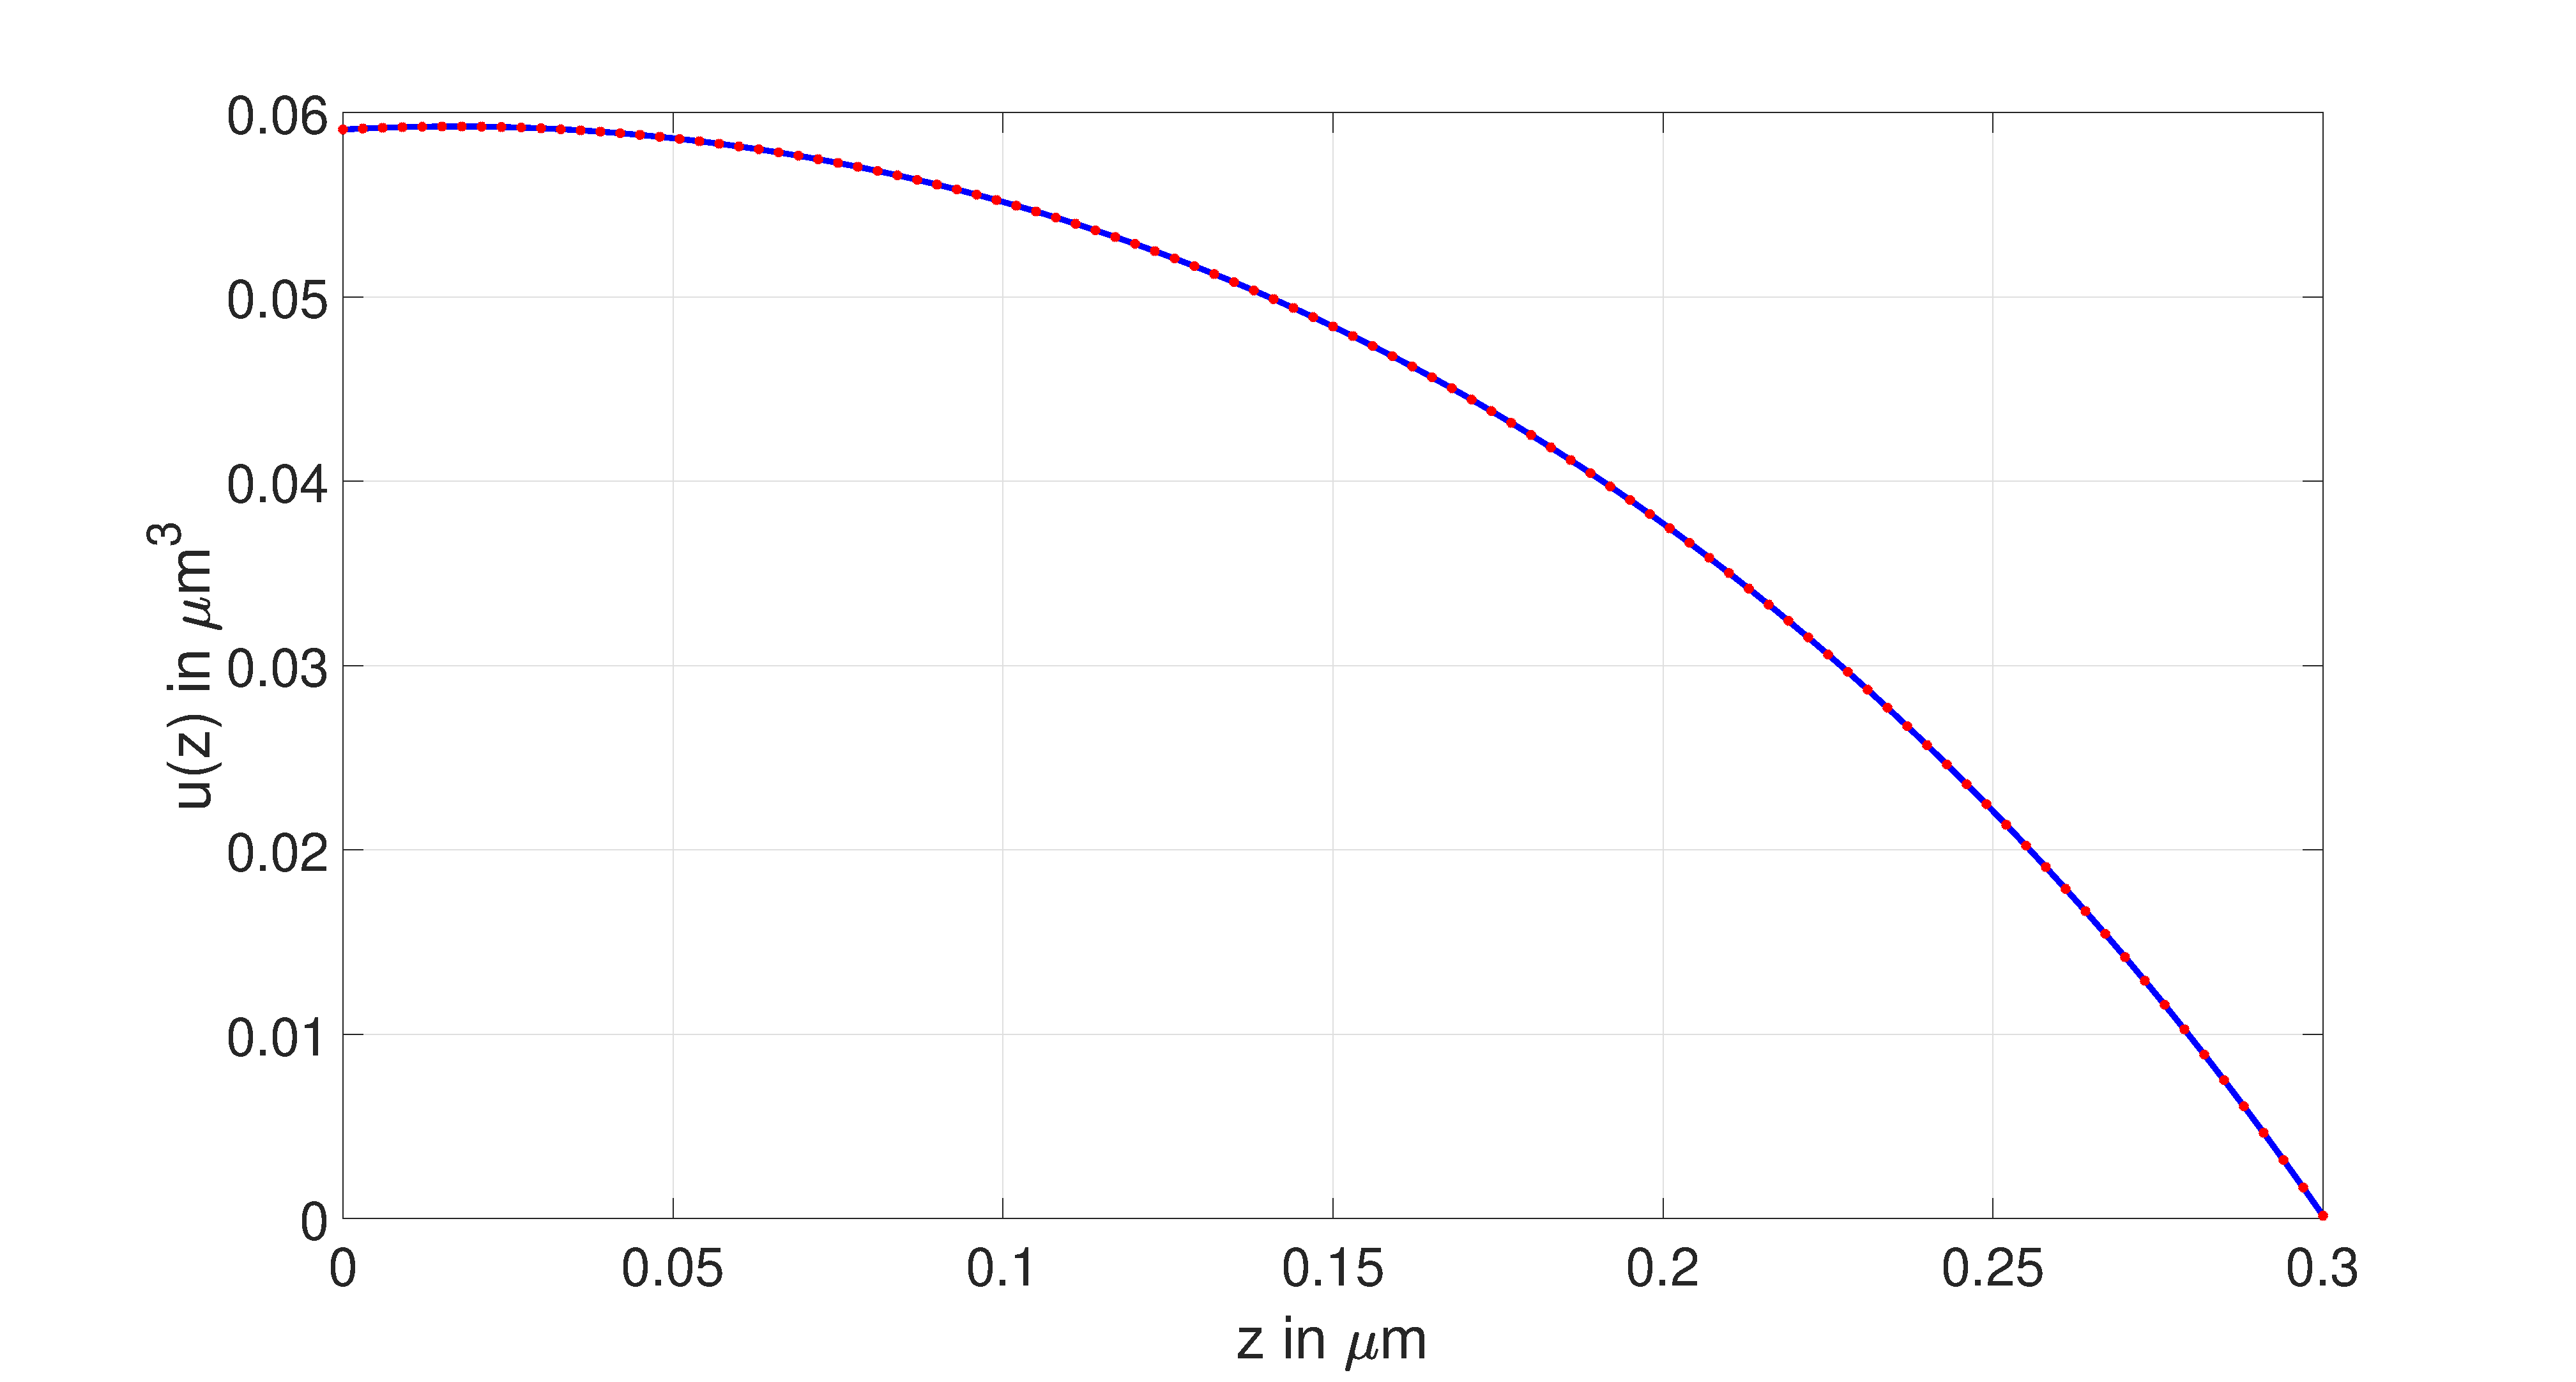
\includegraphics[width=1\linewidth]{figures/station_gl_2_1/aufgabe_7_test_100}
		\caption{Testfunktion
			$\vec{s}(z_\mathrm{i})=\vec{e_\mathrm{i}}$ für $N=100$}
		\label{fig:aufgabe7test}
	\end{subfigure}
	\begin{subfigure}[b]{.5\textwidth}
		\centering

		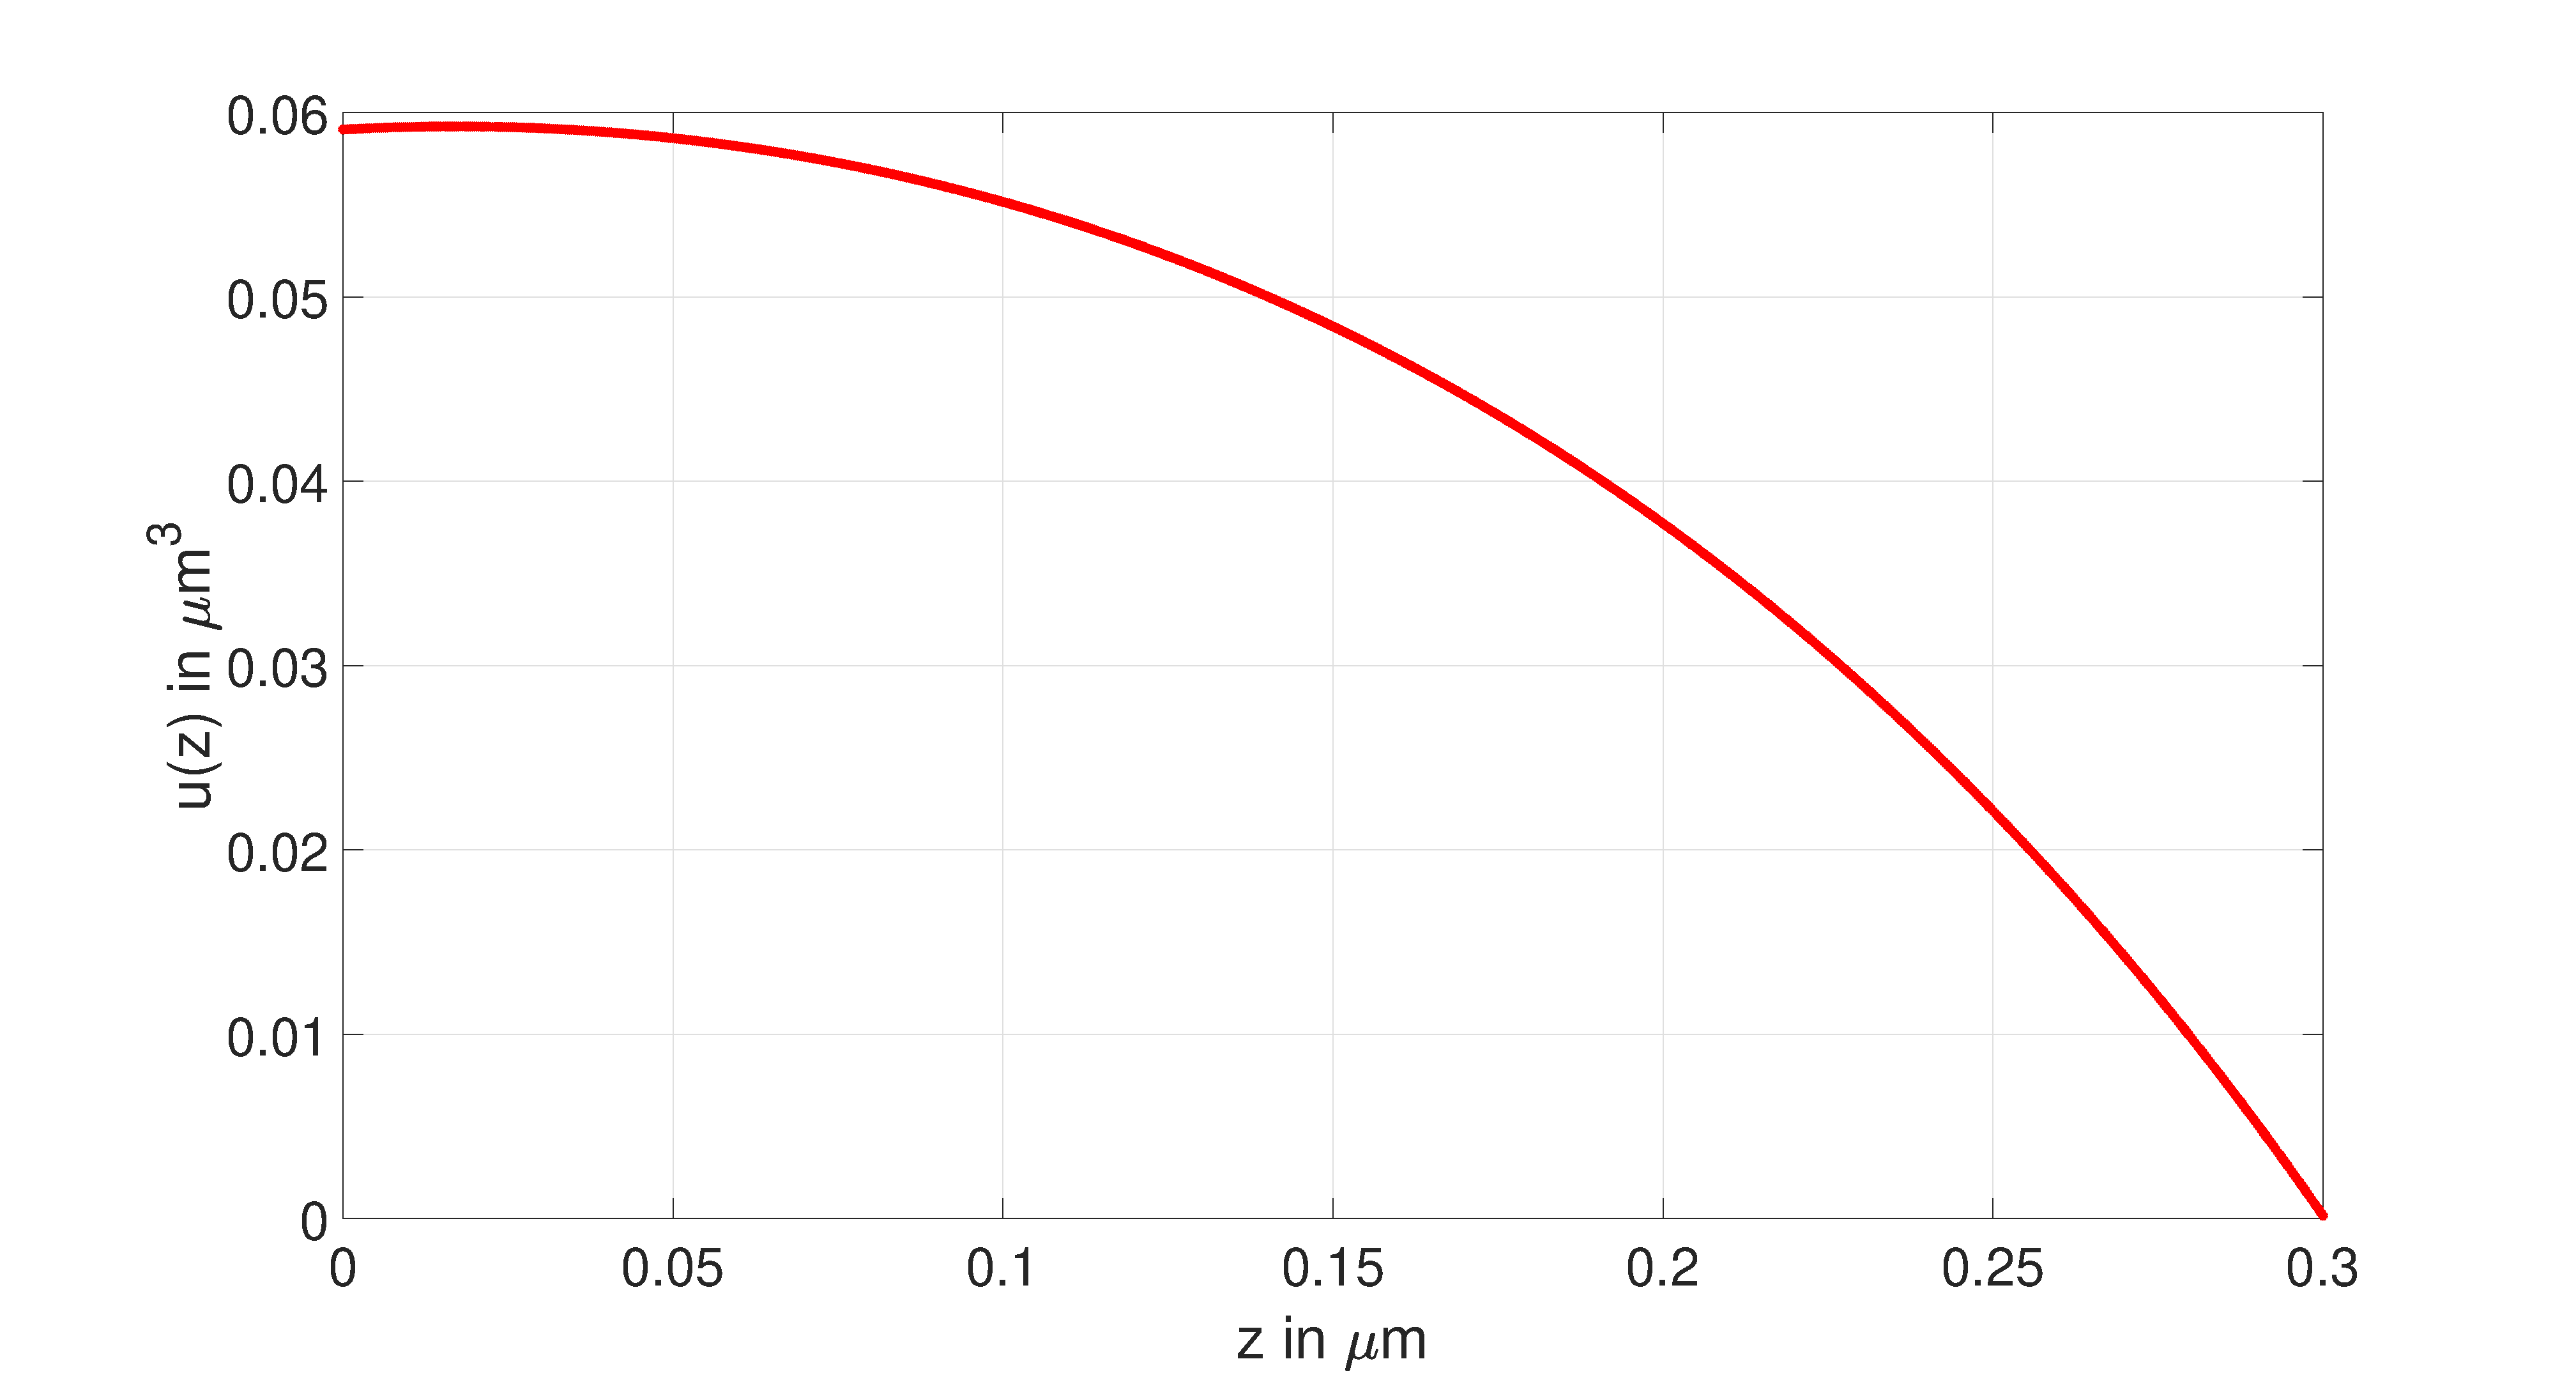
\includegraphics[width=1\linewidth]{figures/station_gl_2_1/aufgabe_7_test_n1000}
		\caption{Testfunktion
			$\vec{s}(z_\mathrm{i})=\vec{e_\mathrm{i}}$ für $N=1000$}
	\end{subfigure}
	\newline
	\begin{subfigure}[b]{.5\textwidth}
		\centering

		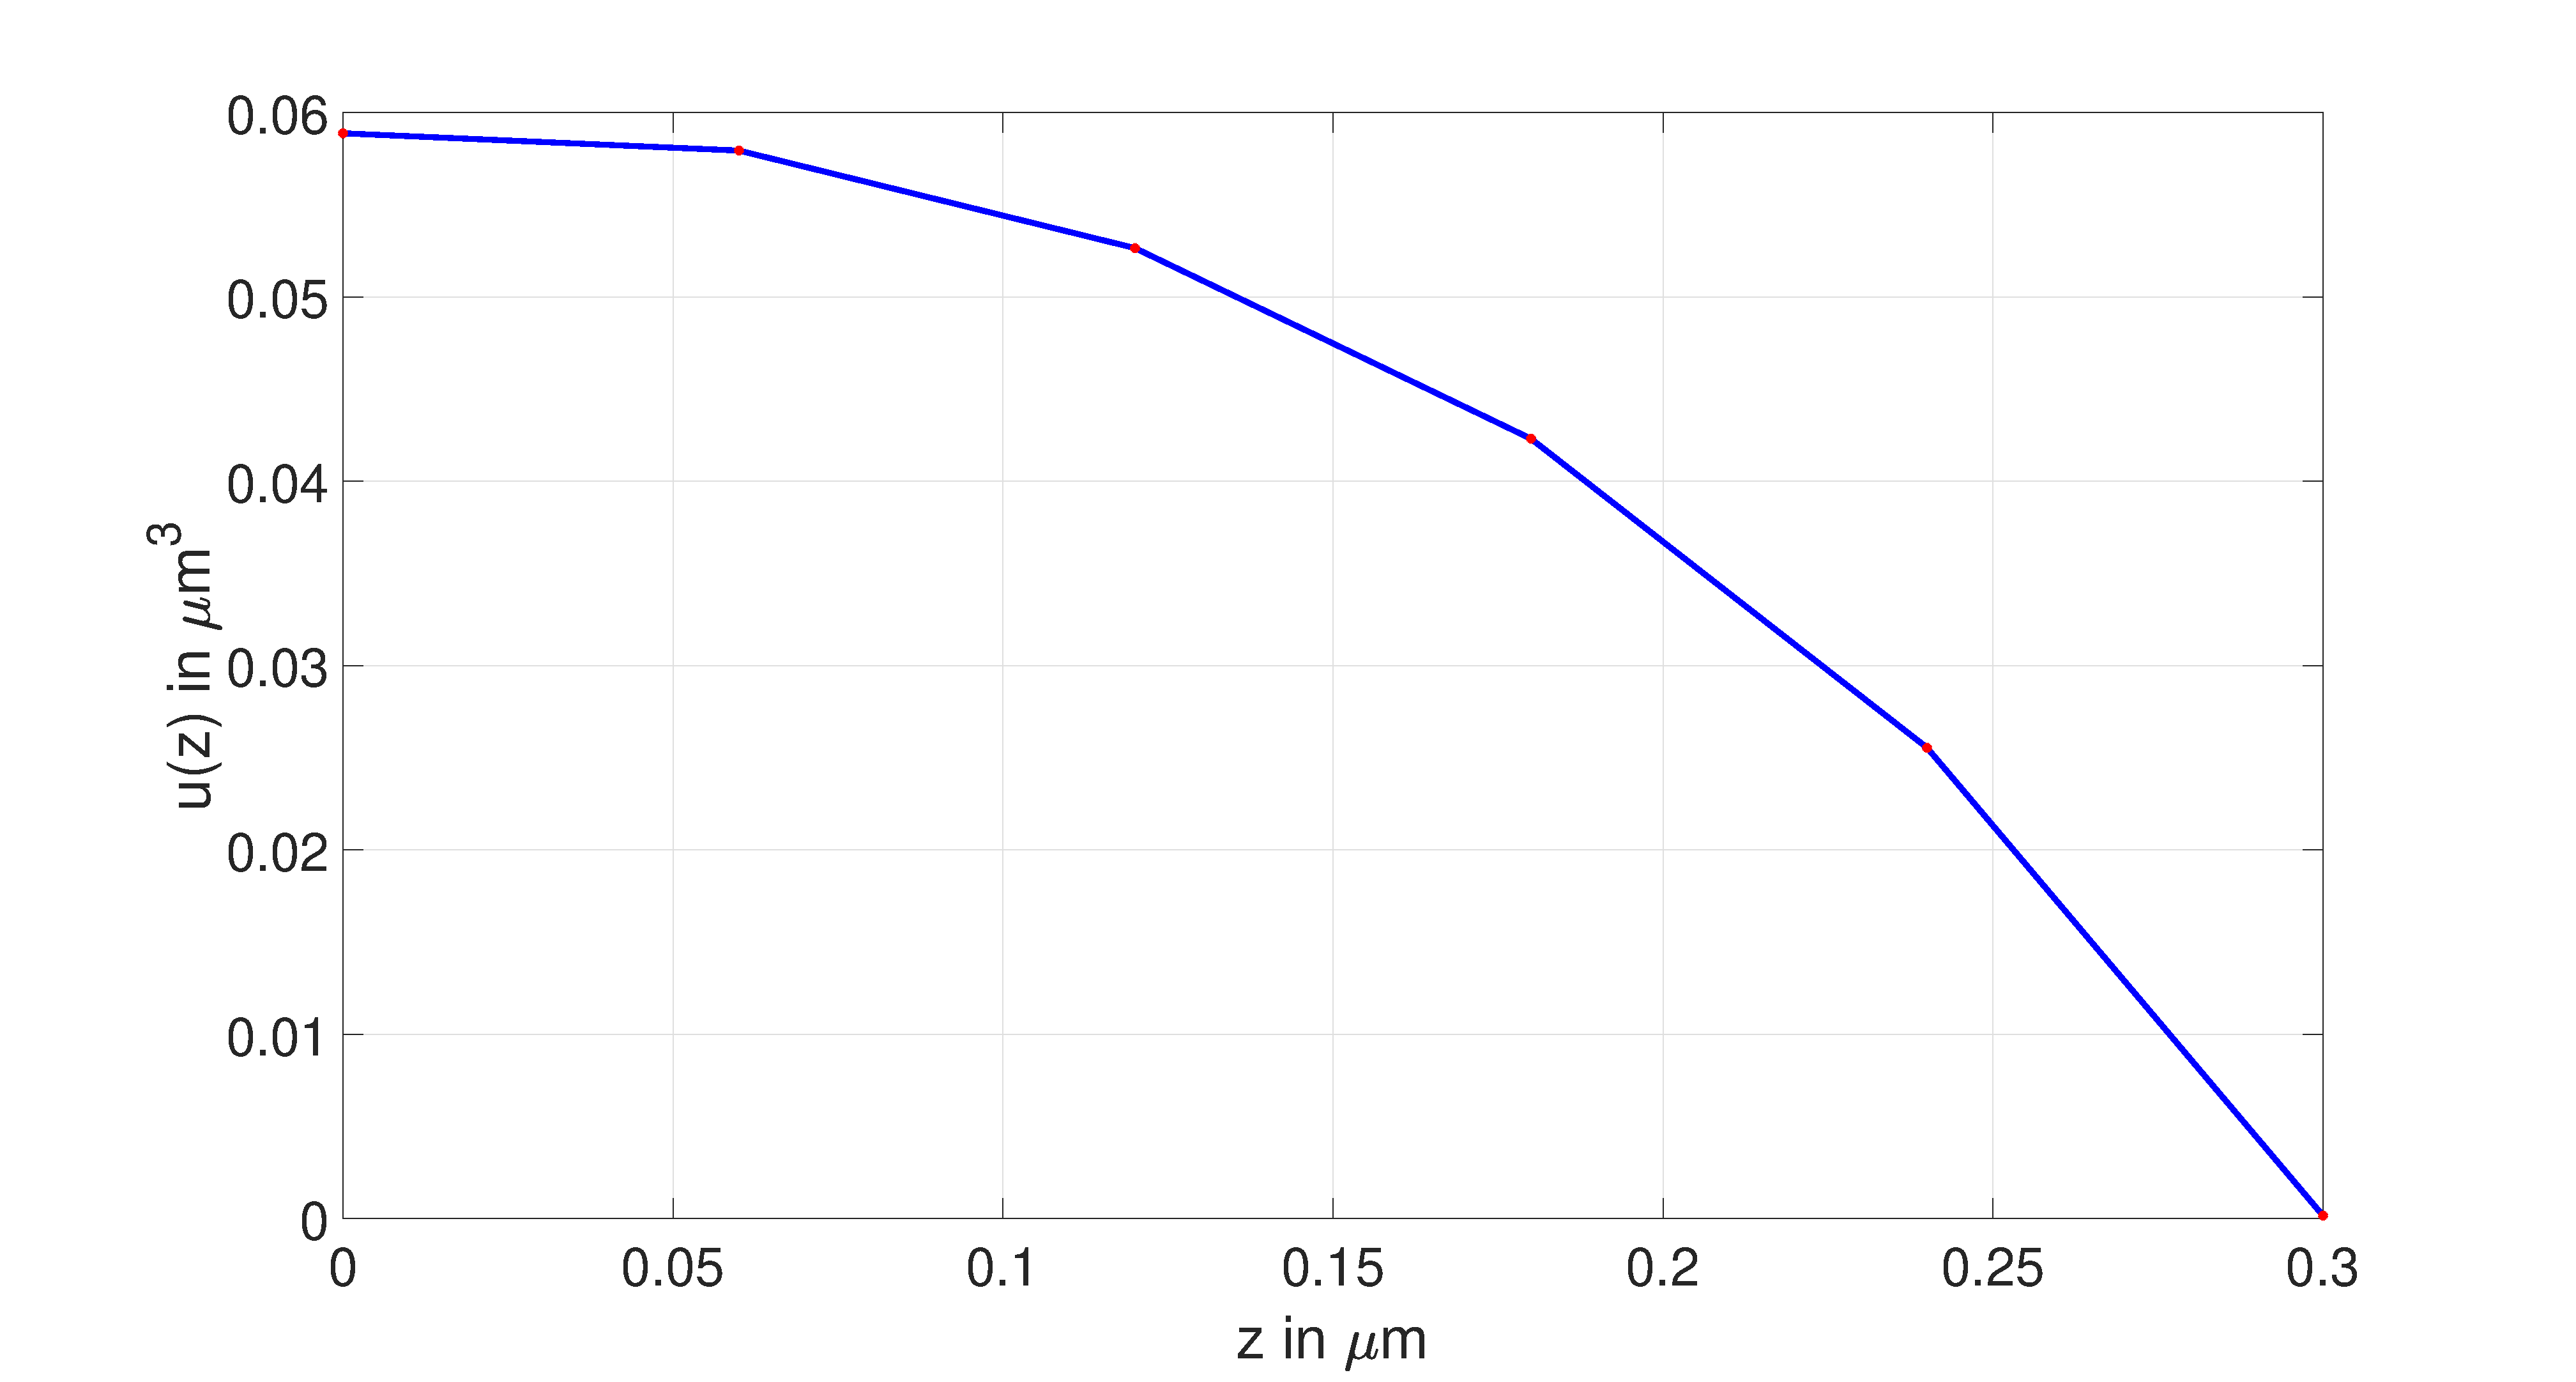
\includegraphics[width=1\linewidth]{figures/station_gl_2_1/aufgabe_7_test_n5}
		\caption{Testfunktion $\vec{s}(z_\mathrm{i})=\vec{e_\mathrm{i}}$ für
			$N=5$}
	\end{subfigure}
	\begin{subfigure}[b]{.5\textwidth}
		\centering

		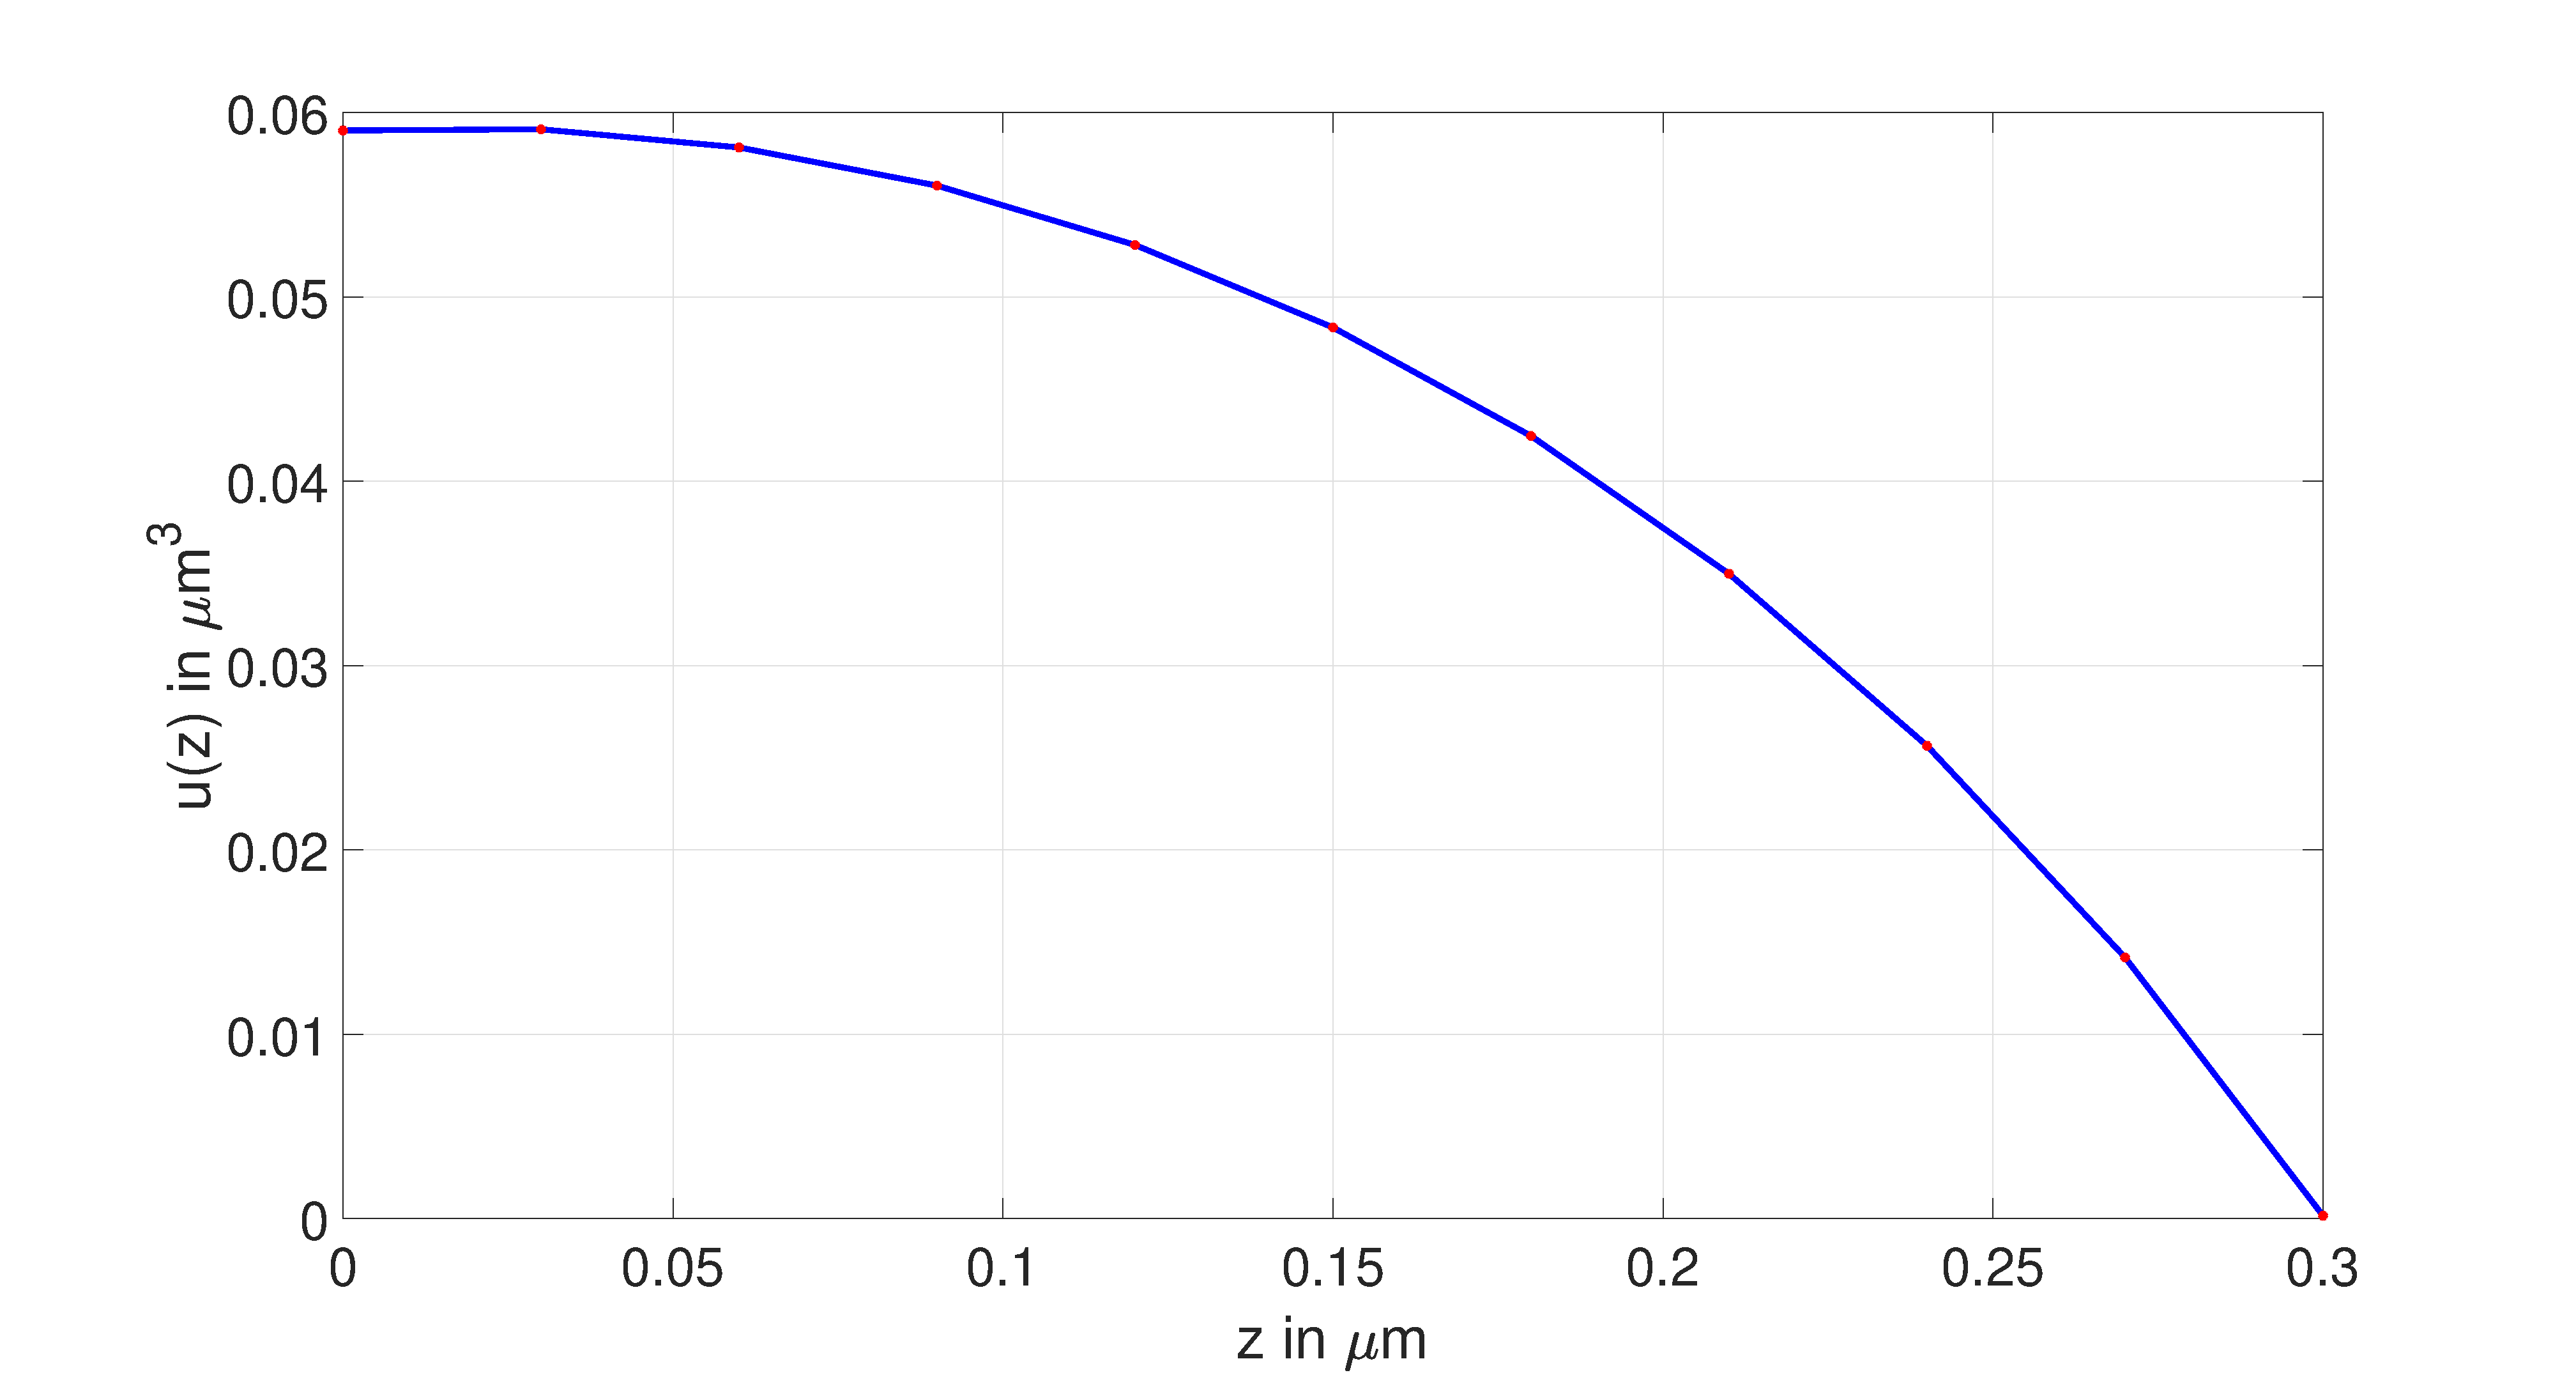
\includegraphics[width=1\linewidth]{figures/station_gl_2_1/aufgabe_7_test_n10}
		\caption{Testfunktion $\vec{s}(z_\mathrm{i})=\vec{e_\mathrm{i}}$ für
			$N=10$}
	\end{subfigure}
\end{figure}
\begin{mybox}
	\textbf{Aufgabe 7. :}	Berechnen Sie mit Hilfe der obigen Routine die Lösung
	für die Fälle
	\begin{equation}
		s(z)=S_0\cdot e^{-\alpha z}, \quad S_0=10^2, \, 10^2, \, 10^4
		\frac{1}{\si{\mu\meter^3 \mu \s}}
	\end{equation}
	Bestimmen Sie näherungsweise experimentell ein geeignetes $N$, so dass der
	relative Fehler in $u_i$
	maximal $1\%$ beträgt, und stellen Sie die Lösung graphisch dar.
\end{mybox}
\begin{figure}

	\lstinputlisting[style=Matlab-editor,caption={Testfunktion}]{Matlab_files/test_2_1.m}
\end{figure}

\section{Nicht Lineare stationäre Gleichung}
\begin{mybox}
	Im zweiten Schritt soll nun die volle nichtlineare \cref{eq:stationDGL}
	mit Randbedingung \cref{eq:randbedingungen} gelöst werden. Analog
	zum letzten Abschnitt wird ein nichtlineares Gleichungssystem
	aufgestellt, das mithilfe des Newton-
	Verfahrens aus der Belegarbeit gelöst werden soll. Gehen Sie wie folgt
	vor.\cite{Prof.Dr.AndreasZeiser.April2021}
\end{mybox}

\begin{mybox}
	\textbf{Aufgabe 1. :} Leiten Sie die nichtlinearen Gleichungen für die
	gesuchten Werte $u_0,u_1,\dots ,uN$ her und stellen Sie
	sie in Form
	\begin{equation*}
		\tcbhighmath{\mathbf{F}(\mathbf{u})=\mathbf{b}}
	\end{equation*}
	dar. Berücksichtigen Sie die Randbedingungen wie im letzten Abschnitt.
	\cite{Prof.Dr.AndreasZeiser.April2021}
\end{mybox}
Nichtlineare DGL:
\begin{equation}
	D\pdv[2]{u}{z}-(k_1+k_2N_D)u-k_2u^2=-s(z)
\end{equation}

Diskretisierung der DGL:

\begin{equation}
	D\frac{u_{i+1}-2u_i+u_{i-1}}{h^2}-k\cdot u_i-k_2 \cdot u_i^2=z_i
\end{equation}

Mit den Randbedingung:

\begin{equation}
	D\cdot \frac{\partial u}{\partial z}(0)=S_Lu(0),\quad D\frac{\partial
		u}{\partial z}(d)=-S_Ru(d)
\end{equation}

Und den Approximationen der ersten Ableitung der  Randbedingungen:
\begin{equation}
	u'(0)\approx \frac{u_1-u_{-1}}{2h} \quad u'(d)\approx
	\frac{u_{N+1}-u_{N-1}}{2h}
\end{equation}
Damit folgt für die Randbedingung:
\begin{equation}
	D\cdot \frac{u_1-u_{-1}}{2h}=S_Lu_0,\quad
	D\frac{u_{N+1}-u_{N-1}}{2h}=-S_Ru_N
\end{equation}
umgestellt nach $u_{-1}$
\begin{equation}
	u_{-1}=-\frac{S_L 2h}{D}\cdot u_0+u_1
\end{equation}
umgestellt nach $u_{N+1}$
\begin{equation}
	u_{N+1}=-\frac{S_R2h}{D}\cdot u_N+u_{N-1}
\end{equation}

Damit folgt für die Funktion $\mathbf{F}(\mathbf{u})=\mathbf{b}$:

\begin{align*}
	F_0 & = \quad
	\frac{D}{h^2}u_1-\frac{2D+kh^2}{h^2}u_0+\frac{D}{h^2}\cdot\left( -\frac{S_L
	2h}{D}\cdot u_0+u_1\right) -k_2u_0^2                                  \\
	\vdots                                                                \\
	F_i & =	\frac{D}{h^2}u_{i+1}-\frac{2D+kh^2}{h^2}u_i+\frac{D}{h^2}\cdot
	u_{i-1} -k_2u_i^2                                                     \\
	\vdots                                                                \\
	F_N & = \frac{D}{h^2}\left( -\frac{S_R2h}{D}\cdot u_N+u_{N-1}\right)
	-\frac{2D+kh^2}{h^2}u_N+\frac{D}{h^2} u_{N-1}-k_2u^2_N                \\
\end{align*}

\begin{qed}
	Vereinfacht zu :

	\begin{align*}
		F_0 & = \quad 2\cdot \frac{D}{h^2}u_1-\ \frac{S_L2h+2D+kh^2}{h^2}
		u_0 -k_2u_0^2                                                     \\
		\vdots                                                            \\
		F_i & =
		\frac{D}{h^2}u_{i+1}-\frac{2D+kh^2}{h^2}u_i+\frac{D}{h^2}\cdot u_{i-1}
		-k_2u_i^2                                                         \\
		\vdots                                                            \\
		F_N & =
		-\frac{2D+kh^2+S_R2h}{h^2}u_N+2\frac{D}{h^2}u_{N-1}-k_2u^2_N      \\
	\end{align*}
\end{qed}

\begin{mybox}
	\textbf{Aufgabe 2. :} Implementieren Sie eine Routine zur Berechnung
	von $\mathbf{F}$ der letzten Teilaufgabe.\cite{Prof.Dr.AndreasZeiser.April2021}
\end{mybox}

\begin{figure}[htb]
	\lstinputlisting[style=Matlab-editor]{Matlab_files/fd_nonlin.m}
\end{figure}

\begin{mybox}
	\textbf{Aufgabe 3. :} Berechnen Sie die Jacobi-Matrix $D\mathbf{F}$ von
	$\mathbf{F}$ bezüglich u und geben Sie sie an
\end{mybox}
\begin{equation}
	J_\mathrm{F}(u)=
	\begin{bmatrix}
		\pdv{F_0(u)}{u_0} & \pdv{F_0(u)}{u_1} & \dots  &
		\pdv{F_0(u)}{u_\mathrm{N}}                              \\
		\pdv{F_1(u)}{u_0} & \pdv{F_1(u)}{u_1} & \dots  &
		\pdv{F_1(u)}{u_\mathrm{N}}                              \\
		\vdots            & \vdots            & \vdots & \vdots \\
		\pdv{F_N(u)}{u_0} & \pdv{F_N(u)}{u_1} & \dots  &
		\pdv{F_N(u)}{u_\mathrm{N}}

	\end{bmatrix}
\end{equation}

\begin{align}
	 & DF(u)\mathrm=                                                  \\
	 & \begin{bmatrix}
		   -	\frac{S_L2h+2D+kh^2}{h^2}-2\cdot k_2u_0 &
		   2\cdot \frac{D}{h^2}                     &                                                                              \\
		   \frac{D}{h^2}                            & \frac{2D+kh^2}{h^2}-2\cdot k_2
		   u_\mathrm{1}                             & \frac{D}{h^2}                                                                \\
		                                            & \ddots                         & \ddots                           & \ddots & \\
		                                            & \frac{D}{h^2}                  & - \frac{2D+kh^2}{h^2}-2\cdot k_2
		   u_\mathrm{N-1}                           & \frac{D}{h^2}                                                                \\
		                                            &                                & 2\frac{D}{h^2}                   &
		   -\frac{2D+kh^2+S_R2h}{h^2}-2\cdot k_2u_N                                                                                \\
	   \end{bmatrix}
\end{align}

\begin{mybox}
	\textbf{Aufgabe 4. :}Implementieren Sie eine Routine zur Berechnung der
	Jacobi-Matrix $DF$ von $F$ der letzten Teilaufgabe.
	Verwenden Sie dabei dünnbesetzte Matrizen.
\end{mybox}

\lstinputlisting[style=Matlab-editor]{Matlab_files/fd_nonlin_jac.m}

\begin{mybox}
	\textbf{Aufgabe 5. :}
	Implementieren Sie eine Routine zur Lösung des Gleichungssystems (8)
	unter Verwendung \verb*|fd_nonlin|
	und \verb*|fd_nonlin_jac| und des Newton-Verfahrens wie in der
	Belegaufgabe. Wählen Sie einen geeigneten
	Startwert.
\end{mybox}
\lstinputlisting[style=Matlab-editor]{Matlab_files/stationaer_nonlin.m}

\begin{mybox}
	\textbf{Aufgabe 7. :}	Berechnen Sie mit Hilfe der obigen Routine die
	Lösung für die Fälle
	\begin{equation}
		s(z)=S_0\cdot e^{-\alpha z}, \quad S_0=10^2, \, 10^2, \, 10^4
		\frac{1}{\si{\mu\meter^3 \mu \s}}
	\end{equation}
	Bestimmen Sie näherungsweise experimentell ein geeignetes $N$, so dass
	der relative Fehler in $u_i$
	maximal $1\%$ beträgt, und stellen Sie die Lösung graphisch
	dar.Vergleichen Sie die Lösung mit den
	entsprechenden Lösungen der linearen Gleichung.
\end{mybox} \clearpage
\chapter{Implizite Einschrittverfahren}
In diesem Kapitel werden Methoden zur Lösung von sogenannten steifen Anfangswertproblemen behandelt. 
Dazu soll Folgendes Chemisches Problem anhand einer DGL untersucht werden.

Die zu untersuchenden Reaktionsgleichungen sind:
\begin{equation}
	A\rightarrow B, \quad B+B \rightarrow C+B, \quad B+C\rightarrow A+C
\end{equation}

Die Dynamik der Konzentrationen der Komponenten werden durch folgende Anfangswertprobleme beschrieben:
\begin{align*}
	A:y'_1&= &{}-0.04\cdot y_1  &{}+ 10^4\cdot y_2y_3& & &\\
	B:y'_2&= & 0.04\cdot y_1  &{}- 10^4\cdot y_2y_3& &{}- 3\cdot 10^7y_2^2 &\\
	C:y'_3&= &                  &                  &  & 3\cdot 10^7y_2^2 &\\
\end{align*}
mit den Anfangswerten 


\section{Entwicklung}
\section{Anwendung}



 \clearpage
%Anhang
\pagenumbering{Alph}

%Abbildungsverzeichnis
\listoffigures \clearpage
%Tabellenverzeichnis
%\listoftables \clearpage
%Quelltextverzeichnis
%\lstlistoflistings \clearpage
%Stichwortverzeichnis
%\printindex \clearpage
%Glossar
%\printglossary[title={Glossar}] \clearpage
%Abkürzungsverzeichnis
%\printglossary[style=dottedlocations,type=\acronymtype,title={Abkürzungsverzeichnis}] \clearpage

%Literaturverzeichnisse (getrennt nach Stichwort)
%\printbibliography[heading=bibintoc, keyword={book}, %title={Literaturverzeichnis}]\clearpage
%\printbibliography[heading=bibintoc, keyword={online}, title={Onlinequellen}]\clearpage
%\printbibliography[heading=bibintoc, keyword={image}, title={Bildquellen}]\clearpage
\printbibliography
% Anhang
\appendix

\chapter{}
\addcontentsline{toc}{chapter}{Anhang A}

\section{Diagramm}

\section{Tabelle}

\section{Screenshot}

\section{Graph}

% Eigenständigkeitserklärung
%\addchap{Eigenständigkeitserklärung}

Hiermit versichere ich, dass ich die vorliegende Masterarbeit selbstständig und nur unter
Verwendung der angegebenen Quellen und Hilfsmittel verfasst habe. Die Arbeit wurde bisher
in gleicher oder ähnlicher Form keiner anderen Prüfungsbehörde vorgelegt.

\vskip 1cm

Stadt, den xx.xx.xxxx

\vskip 1.5cm

Max Mustermann

\end{document}